
%
% foundations - mapping
%

\section{Web Mapping}

Maps have become an almost instinctive way of seeing our world. They probably first appeared over 18,000 years ago and already in the 1500s, they were produced in large numbers for navigational and military purposes. Maps are powerful tools that help organize boundaries and administrative activities. They allow telling stories, visualizing data and understanding geographic contexts
~\cite{Zzolo11mappingdrupal}.

Recently, Google Maps\footnote{\url{http://maps.google.com}} has made digital maps available to a large number of internet users. Digital natives are used to navigate using interactive maps on their smart phones and look up places on online maps on their computers.

Web mapping describes the whole process of designing, implementing, generating and delivering maps on the internet. It applies theoretical foundations from web cartography to the technical possibilities and boundaries of constantly evolving web technologies. The continuous development of related technologies has created a wide variety of \textit{types of web maps}: from analytic, animated, collaborative and dynamically created web maps to online atlases, realtime and static web maps~\cite{wiki:web-mapping}.

In order to represent spatial locations, \textit{reference systems} are used that subdivide the geographic area into units of common shape and size. Such spatial reference systems consist of a \textit{coordinate system}, a \textit{datum} and a \textit{projection}. \textit{Geodetic datums} are models that approximate the shape of the Earth. In the following two chapters, the remaining concepts of coordinate systems and map projections will be explained in more detail.

\subsection{Coordinate systems}

In mapping, a coordinate system is used to represent spatial locations in a numeric way. We mainly differentiate between \textit{Cartesian} and \textit{Ellipsoidal} coordinate systems. 

\begin{itemize}

\item \textbf{Cartesian coordinate systems} express a spatial location by specifying the distances to the axes. The axes are usually labeled $X$, $Y$ and $Z$ for locations in three-dimensional space. As an example, the \textit{Earth Centered, Earth Fixed X, Y, and Z (ECEF)} coordinate system is used by positioning technologies such as GPS. The coordinates of New York in ECEF are:

\[ (X, Y, Z) = (1334.409~km, -4653.636~km, 4138.626~km) \]

``Earth centered'' emphasizes that the origin of the axes is defined to be at the geocenter of the planet. This system isn't intuitive when referencing points sd the values don't indicate if a location is on above or below the surface of the Earth. 

\item \textbf{Ellipsoidal coordinate systems} describe a more convenient way of expressing spatial location on the Earth's surface. A \textit{reference ellipsoid} approximates the shaper of the Earth by an equatorial and a polar radius. As a result, positions at the surface of the Earth can be represented angles. This defines the primary way of expressing coordinates as a pair of \textit{latitude} and \textit{longitude} values.

  \begin{itemize}

  \item \textbf{Latitude} classifies the angular distance towards north and south from the equator which is at $0^\circ$. Positive latitude values represent the northern hemisphere up the the pole at $90^\circ$. Negative values are located below equator where the south pole marks the lower limit at $-90^\circ$.

  \item \textbf{Longitude} denotes the angular distance towards west and east. It's zero-mark is a latitude of $0^\circ$  which runs north-south through the Royal Observatory at Greenwich in the UK. In contrast to latitude values, the longitude encloses a whole circle around the earth. Negative values down to $180^\circ$ are located west and positive values up to $180^\circ$ are positioned east of Greenwhich.

  \end{itemize}

In classic mapping applications, latitude and longitude values are measured in degrees, minutes and seconds of the sphere. New York City is located at $40^\circ$ $43'$ $0''$ North, $74^\circ$ $0'$ $0''$ West. For computational purposes, web mapping is largely based on a decimal degree representation of such values. The equivalent decimal degree value for New York in that case is the pair of

  \[ (latitude, longitude) = (40.716667, -74) \]

A common pitfall in web mapping is mixing up the order of latitude and longitude values. Having latitude before longitude is the standard, which means to state the vertical position before the horizontal. This contradicts with classic Cartesian x,y coordinate systems and often leads to confusion. Some mapping APIs expect latitude first, while others are designed to begin with longitude values~\cite{Kupper2005lbs, Zzolo11mappingdrupal}. 

\end{itemize}




\subsection{Map Projections}

The planet Earth is a roughly spherical geoid. In order to represent it on flat computer screens, the surface of the Earth needs to be translated to a plane. This is realized by applying the method of a map projection which projects the bended, three-dimensional surface of the Earth onto a two-dimensional projection surface. The shape of the projection surface defines different possibilities of projection types as \textit{planar}, \textit{conical} and \textit{cylindrical}. See figure \ref{fig:map-projection-types} for a visual comparison of map projection types.

\begin{figure}[h]
  \begin{center}
    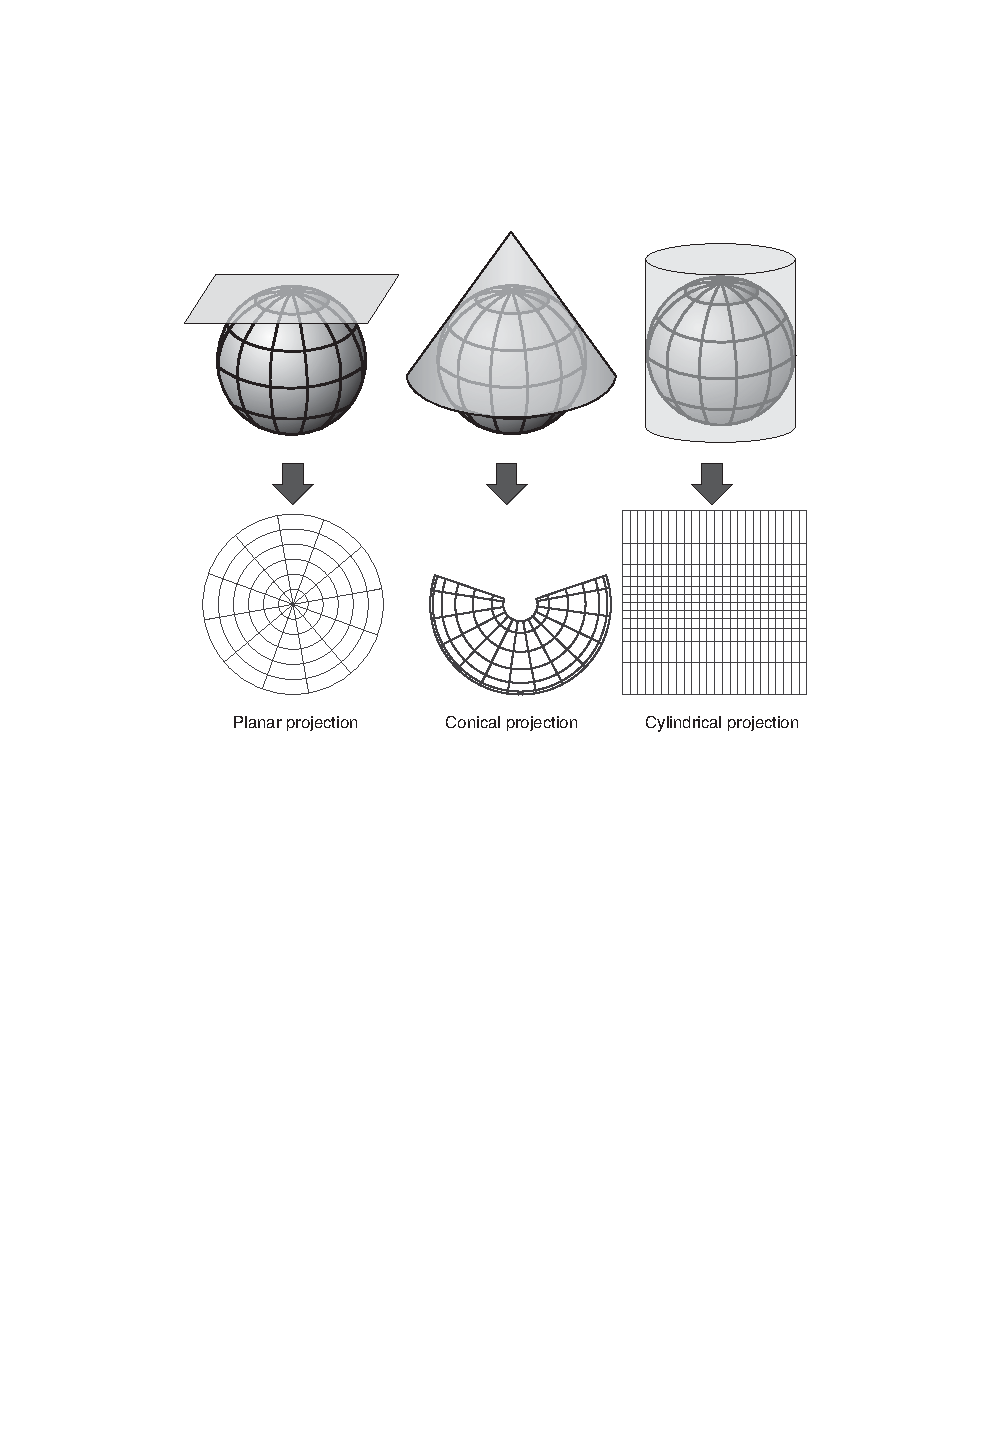
\includegraphics[width=0.75\textwidth]{figures/map_projection_types}
    \caption{Types of map projections~\cite[p 28]{Kupper2005lbs}.}
    \label{fig:map-projection-types}
  \end{center}
\end{figure}

Flattening the curved surface of the Earth naturally causes \textit{distortion} of different kinds including areal, angular, scale, distance and direction distortion. The selection a map projection influences which degree and combination of distortion will be caused. As no projection can optimize all those factors at once, choosing the right projection depends on the purpose of the map.

The \textbf{spherical mercator projection} is the most commonly used web mapping projection. Based on a normal cylindrical projection, it preserves local shapes and direction, but does this at the cost of enlarging areas towards the poles. As an example Greenland appears on a Mercator map larger than South America, its actual size is on $1/8$ though. The effect of this distortion can be visualized by Tissot's indicatrix. Figure \ref{fig:mercator} shows how circles of the same relative size get extrapolated off the equator by using the mercator projection~\cite{Zzolo11mappingdrupal, wiki:web-mapping, Kupper2005lbs}. 

\begin{figure}[h]
  \begin{center}
    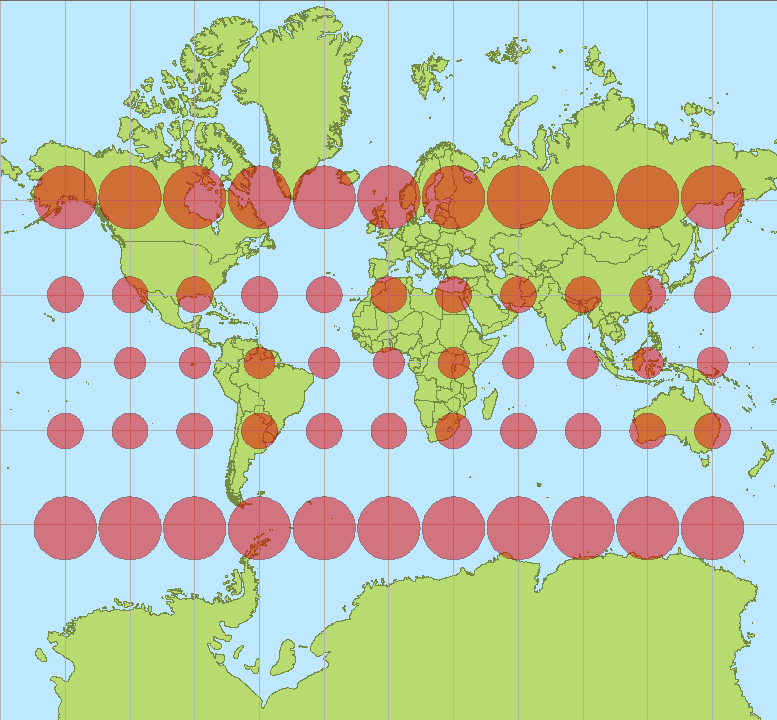
\includegraphics[width=0.65\textwidth]{figures/tissot_mercator.png}
    \caption{Tissot's indicatrix visualizes enlarged areas towards the poles when using the mercator projection~\cite{wiki:mercator}.}
    \label{fig:mercator}
  \end{center}
\end{figure}

Many countries have developed their own coordinate systems such as the British National Grid or the German Gau\ss-Kr\"{u}ger coordinate system. They aim at reproducing the geographic regions within their territory in an appropriate manner. Standardization efforts go towards using the \textit{Universal Transverse Mercator} projection. It avoids large distortions by comprising a series of Transversal Mercator projections that create separate grid zones with their own projections. This has the benefit of universally representing areas in a more exact way. On the other hand, coordinates need to be referenced including the zones in which they are located in~\cite{Kupper2005lbs}.

\subsection{Spatial data types}

Two main representation types for spatial objects such as buildings, roads and other geometries exist: \textit{vector data} and {raster data}. This mainly applies to 2-dimensional representation of spatial data, which often suffices the task for creating web maps and is preferred over 3-dimensional data handling in many cases for computational simplicity. Figure \ref{fig:raster-vector} illustrates the conceptual different between both data types which will be discussed as follows.

\begin{figure}[h]
  \begin{center}
    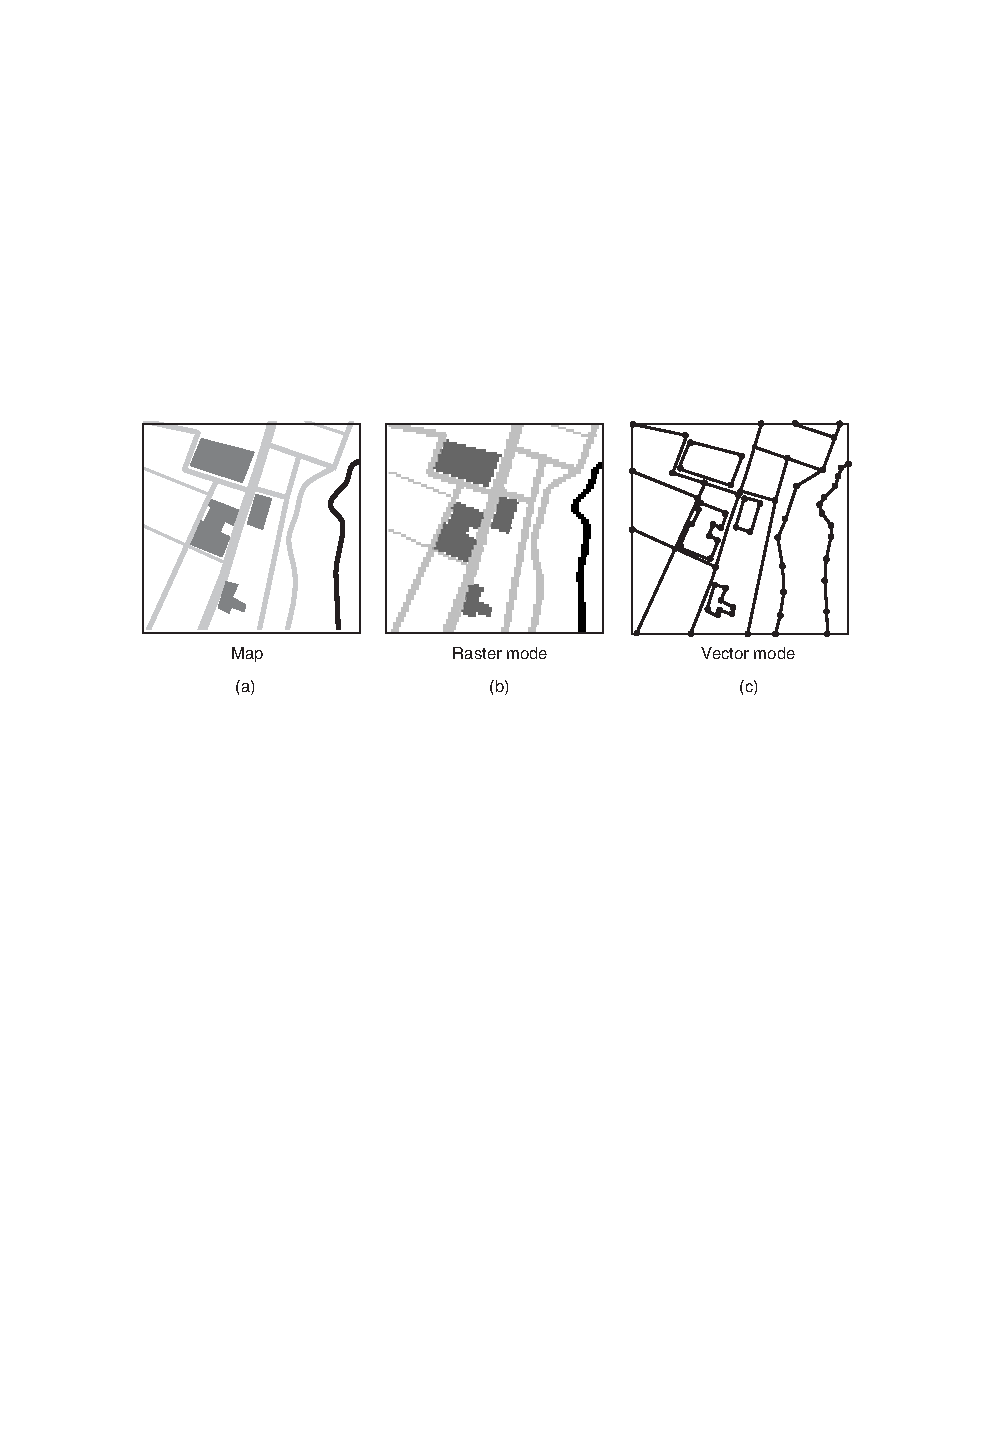
\includegraphics[width=0.9\textwidth]{figures/raster_vs_vector.pdf}
    \caption{A map (a) displayed either in raster mode (b) or in vector mode (c)~\cite[page~38]{Kupper2005lbs}.}
    \label{fig:raster-vector}
  \end{center}
\end{figure}

\begin{itemize}

\item \textbf{Vector data} is used to describe geometric shapes in a numeric way. \textit{Points}, \textit{lines} or \textit{polygons} are specified by coordinates in a reference system.

Simple points can be easily expressed as pairs of latitude, longitude values and stored within two separate columns within a database. More complex shapes like polygons require different data storage types, such as \textit{Well Known Text} (WKT) and \textit{Keyhole Markup Language} (KML).

\item \textbf{Raster data} represents and stores geospatial data as a grid of pixels that forms a continuos surface. Most commonly used for satellite imaginary it is also popular for storing and delivering pre-rendered vector data as tiled images. The arrangement of adjacent pixels intrinsically defines the spatial location of shapes within the raster image in relation to an externally defined reference system.

The pixel values of the raster image usually depict a visual representation of the contained area, but they can also be assigned a specific meaning: The \textit{digital elevation model} (DEM) for example described the average elevation of the mapped area per pixel.

\end{itemize}

~\cite{Kupper2005lbs, Zzolo11mappingdrupal}

\subsection{The Web Mapping Stack}

The primary purpose of web mapping applications is to deliver spatial data in the form of a map to the user. Modern, interactive web mapping applications are based on a concept named \textit{slippy maps}. These maps are brought to the user by a combination of client- and server-side technologies. 

Slippy maps are displayed in a rectangular viewport within the browser handled by a javascript mapping library. The map is visualized dynamically by rendering layers of raster and vector data on top of each other. In addition, slippy maps provide means of interaction to the user such as panning and zooming to update and explore the map. Figure \ref{fig:web-mapping-stack} illustrates the prototype of such a modern web mapping application. Its components will be discussed in the following section.

\begin{figure}[h]
  \begin{center}
    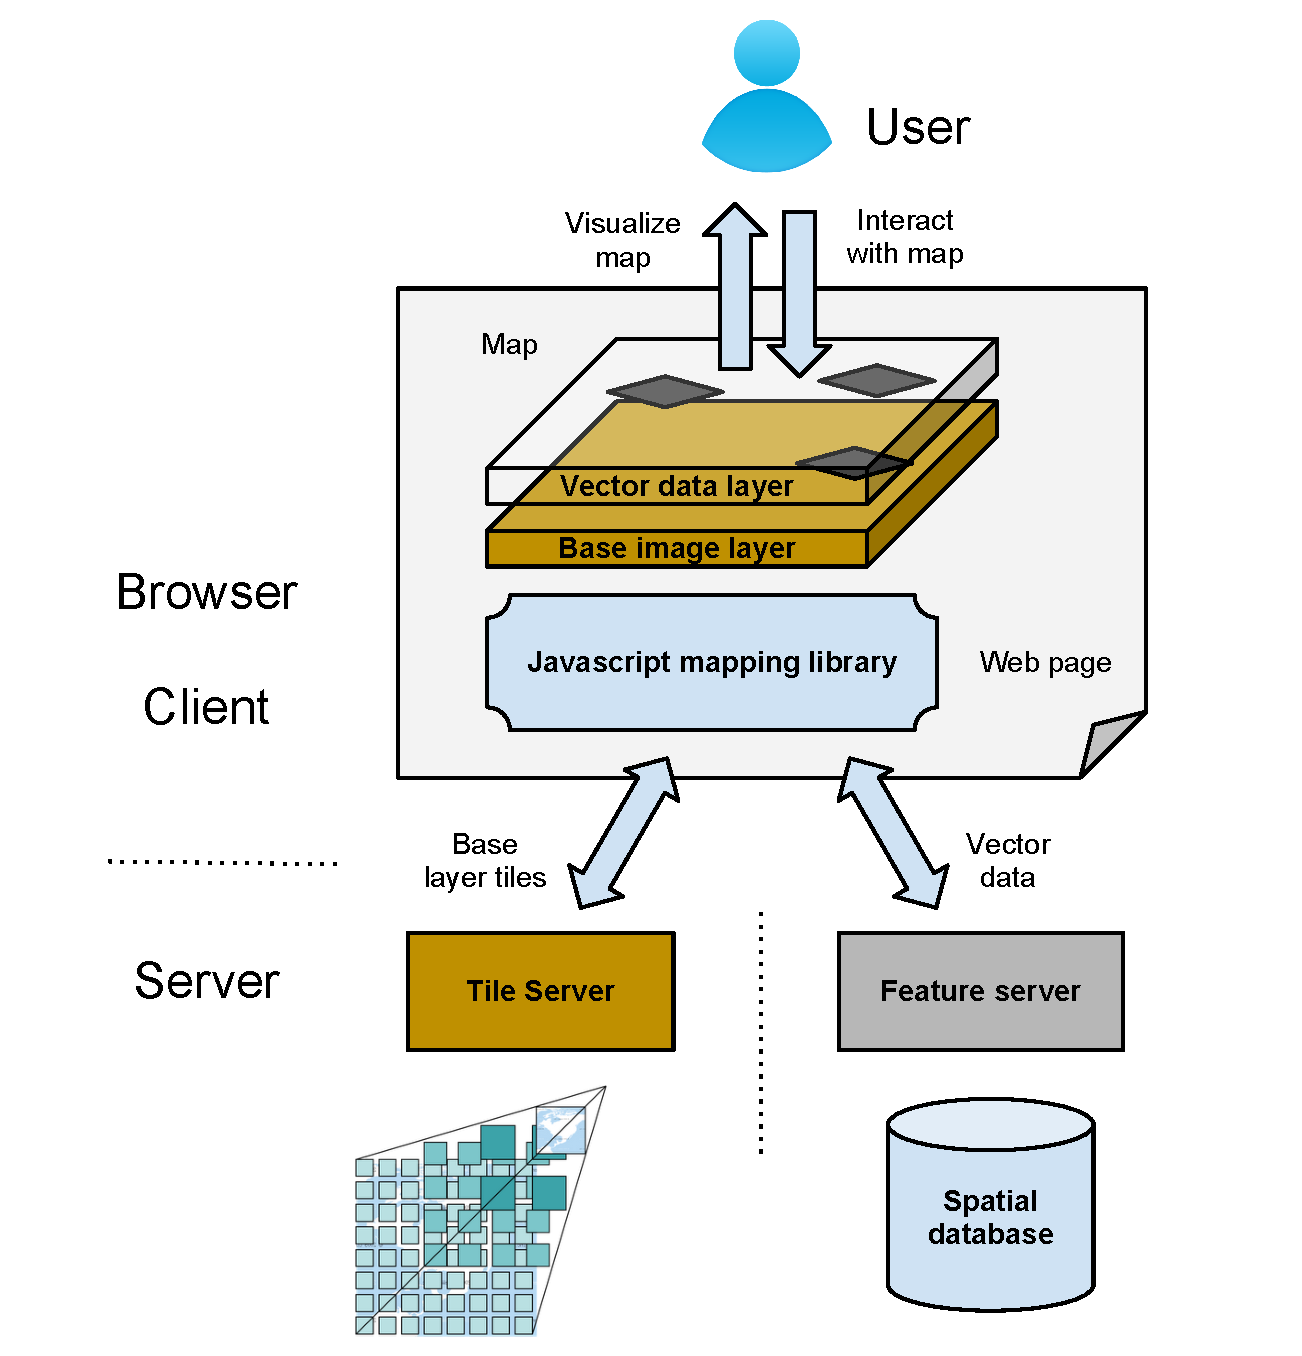
\includegraphics[width=1\textwidth]{figures/web_mapping_stack.pdf}
    \caption{Illustration of a modern web mapping application. Includes a tile graphic from~\cite{web:cubeservtiles}.}
    \label{fig:web-mapping-stack}
  \end{center}
\end{figure}


\begin{itemize}

\item \textbf{Latitude} classifies the angular distance towards north and south from the equator which is at $0^\circ$. Positive latitude values represent the northern hemisphere up the the pole at $90^\circ$. Negative values are located below equator where the south pole marks the lower limit at $-90^\circ$.


\end{itemize}


\cite{Miler10webis}










